\documentclass{scrartcl}
\usepackage[utf8]{inputenc}

\usepackage{gensymb}
\usepackage{caption}
\usepackage{subcaption}
\usepackage{graphicx}
\usepackage{setspace}
\usepackage[margin=1in]{geometry}

\subtitle{Modeling the Collective Behavior of Ants on Uneven Terrain}
\title{Project Description}
\author{Matthew Moreno}

\begin{document}
\maketitle
\section{Project Purpose and Background}
Ant colonies regulate their foraging behavior through a collective decision making process; when ants forage, no individual ant operates with complete information about the terrain being explored. This contrasts with traditional human approaches decision-making, which typically centralize information, process it, then redistribute instructions. Consider, for example, traffic-aware navigation tools such as Waze or Google Maps; the distribution of traffic  across a geographic region is collected from users, centrally processed, and then routing instructions are redistributed to individual users. In contrast, collective intelligence on the level of the ant colony emerges from parallel execution of a simple set of individual pheromone deposit and response behaviors. This distributed decision-making strategy is very effective. Among other feats, foraging ants will tend to choose the shortest path between nest and food and selectively exploit the richest food source when presented with an array of food source choices \cite{camazine_self-organization_2003}.

This summer, I performed research into ant foraging behavior with Professors Simon Garnier and Jason Graham at the New Jersey Institute of Technology. My project focused on extending mathematical models of ant foraging, which are well-developed on flat surfaces, to uneven terrains. On flat terrain, a clear ``best'' path exists: the shortest-distance foraging path and the quickest-trip path are all identical. On uneven terrains, however, this is no longer necessarily the case and the question of which trade-offs ants make -- and how they make them -- is of great interest. After surveying existing models of ant foraging behavior on flat terrain and individual ant behavior on inclined surfaces, I designed and numerically evaluated a differential equations-based model of ant foraging behavior on uneven terrain.

My model will see continued use, enabling the Swarm Lab to work out the rules by which real ants act on uneven terrain in a foraging context by simulating hypothesized behaviors and assessing the resulting foraging path predictions in comparison with \textit{in vivo} ant foraging experiments. Ultimately, research into the collective intelligence of insects translates directly to technological applications. For example, such research has been leveraged in swarm robotics projects, such as NASA's ant-inspired ``Swarmies'' that may one day harvest resources for Martian colonies \cite{falker2015autonomous}

\section{Methods of Study and Findings}
To conduct my research, I designed an individual-based set of differential equations to model \textit{Tetramorium caespitum} foraging behavior over uneven terrain. The design of this model was inspired by existing individual-based differential equations models of ant foraging on flat terrain \cite{perna_individual_2012,ryan_model_2016}. Experimental results describing the behavior of individual ants on uneven terrain -- namely, the effect of incline on ant walking speed \cite{holt_locomotion_2012} and behavioral preference of ants to walk parallel to an incline \cite{khuong_how_2013} -- were incorporated into the model. These additions represent the novel contribution of the research. Figure \ref{fig:model_components} summarizes the components of the mathematical model of ant foraging that was developed.

\begin{figure}[h] 
     \centering
      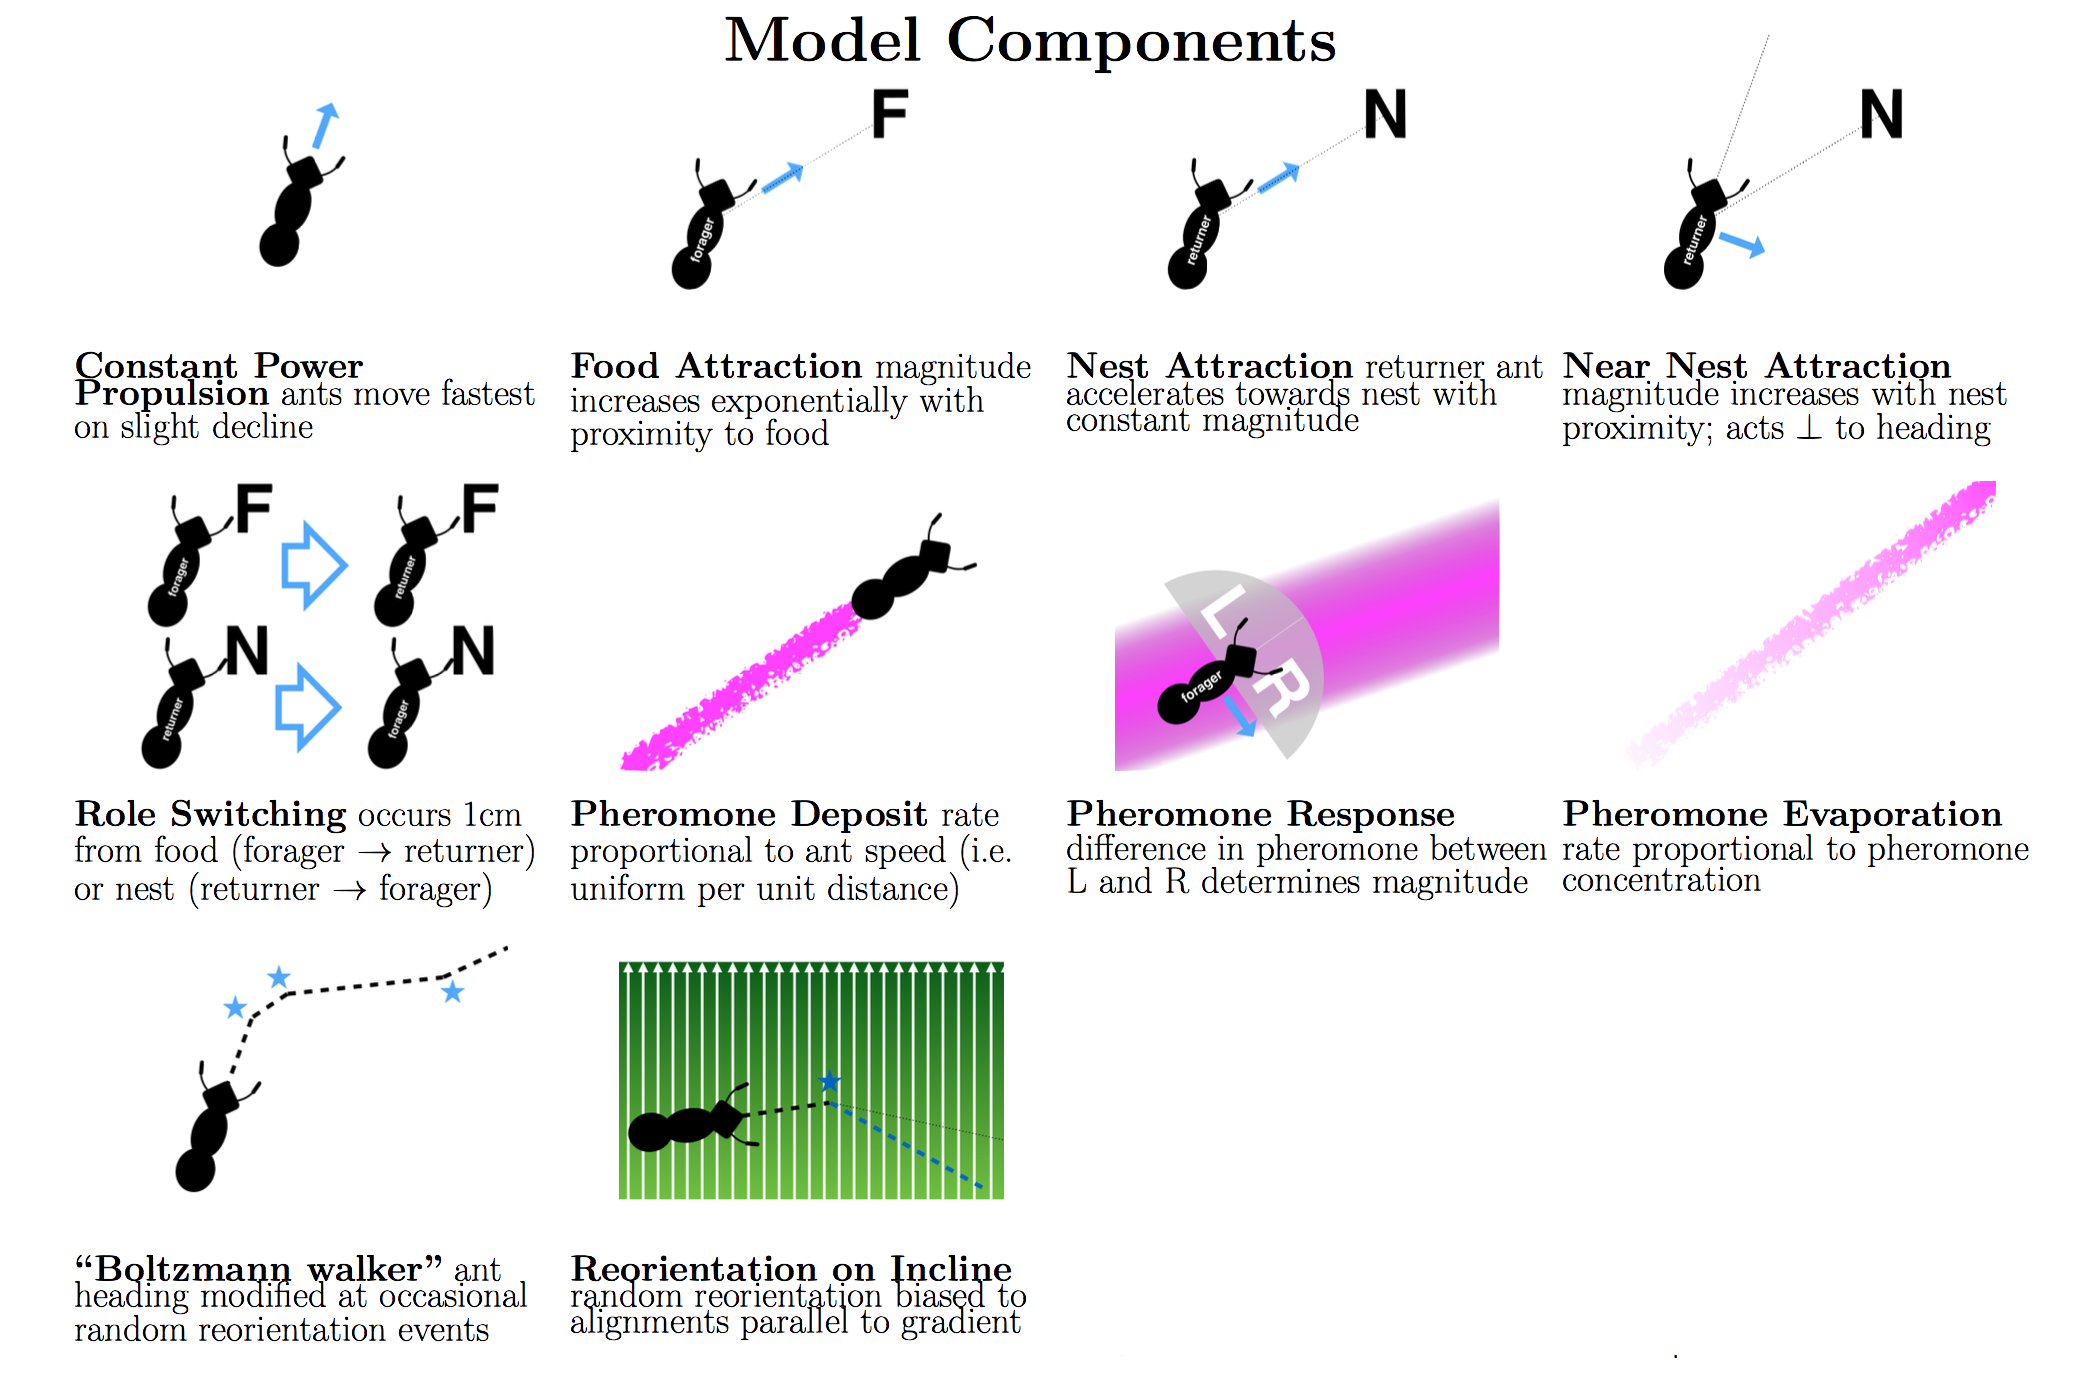
\includegraphics[width=0.8\textwidth]{img/model_components}
      \caption{A visual synopsis of the components of the model of ant foraging}
      \label{fig:model_components}
\end{figure}

The model was implemented to replicate an experimental setup that could be actualized with ants \textit{in vivo} so that the model's predictions can be directly compared to empirical results. The model simulated an ant colony of twenty ants foraging in an enclosed rectangular arena measuring 10cm by 30cm. A 10cm ramp was situated between two 10cm segments of flat terrain. Ant nest and food were placed at opposite ends of the arena along its long axis. Nest and food were placed either in opposite corners or both centered on the arena's short axis. Figure \ref{fig:arena} depicts this experimental setup.

\begin{figure}[h]
  ~
  \begin{subfigure}[b]{0.5\textwidth}
  \centering
  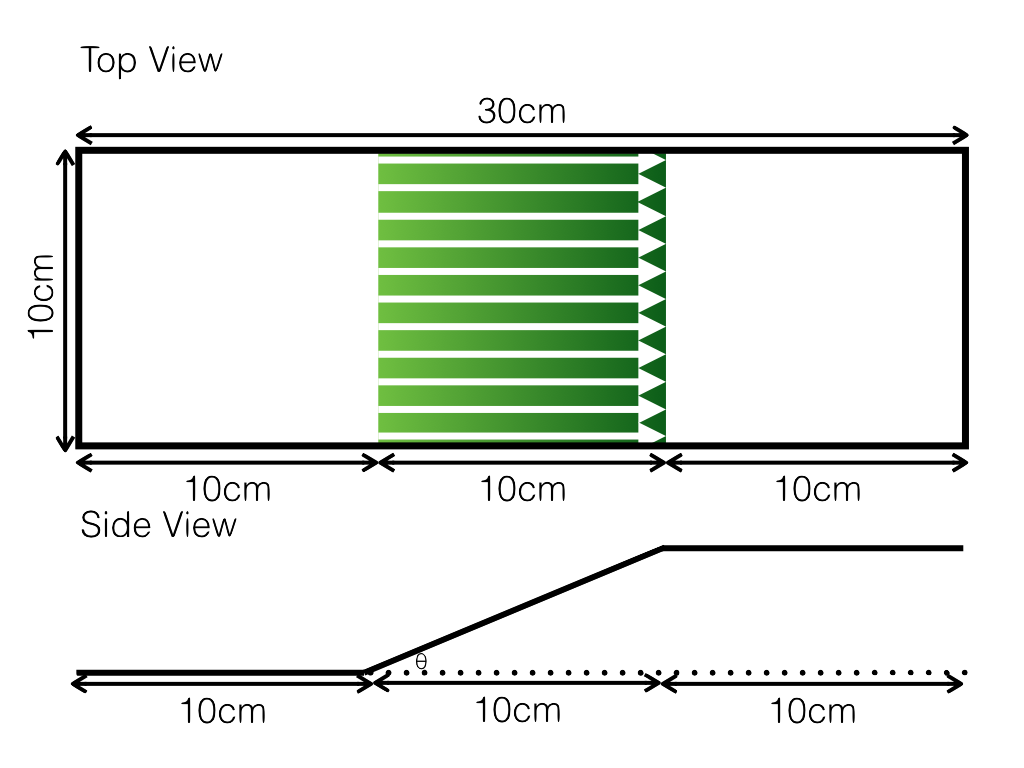
\includegraphics[width=0.8\textwidth]{img/arena_setup}
   \begin{minipage}{0.8\textwidth}
   \subcaption{Arena terrain is comprised of two flat sections joined by a simple incline.}
   \end{minipage}
  \end{subfigure}%
  \begin{subfigure}[b]{0.5\textwidth}
  	\centering
    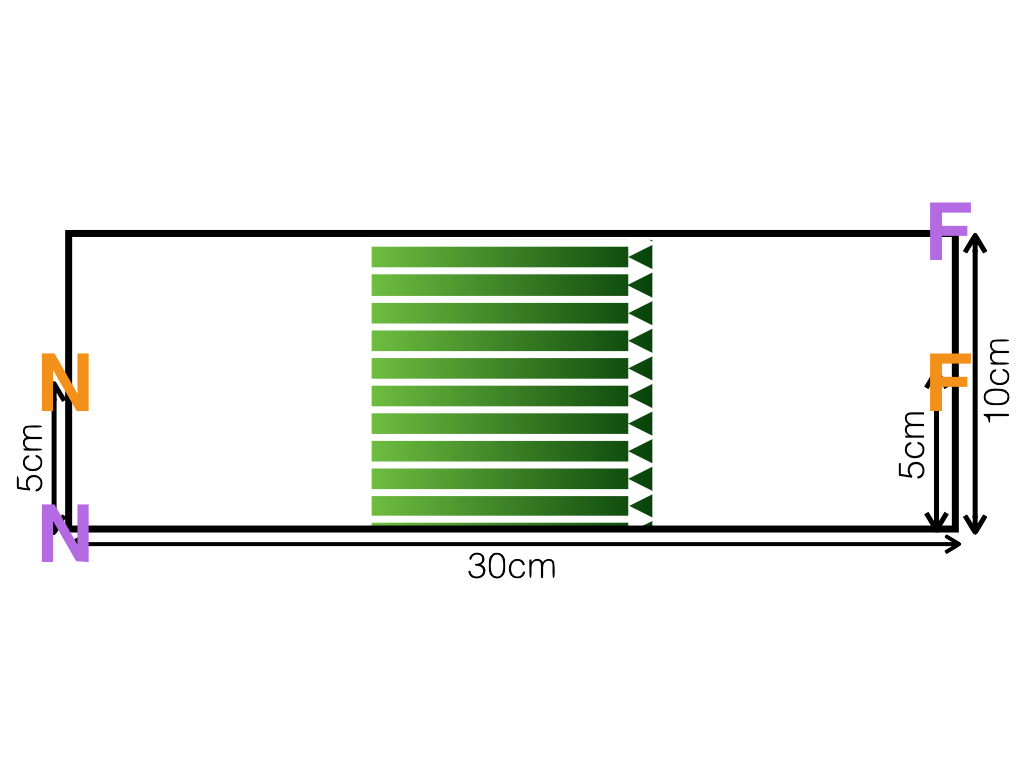
\includegraphics[width=0.8\textwidth]{img/nest_food}
    \begin{minipage}{0.8\textwidth}
    \subcaption{The center-to-center nest/food placement scheme is shown in orange and the corner-to-corner nest/food placement scheme is shown in purple.}
    \end{minipage}
  \end{subfigure}
  \caption{Schematic diagrams illustrating experimental setup} \label{fig:arena}
\end{figure}

Computational experiments were conducted with both nest/food placement schemes and with ramp inclines of $\pm 60\degree$, $\pm 45\degree$, $\pm 30\degree$, and $0\degree$. Numerical solutions of the model predict that as the ramp incline steepens, ants will tend to more strongly favor the direct path between nest and food. That is, the average observed path more closely matches the direct path between food and nest and the foraging path is observed to be less variable over the course of ant foraging. The model predicts these effects of ramp incline on foraging behavior for both the corner-to-corner and center-to-center nest/food placement schemes. 

\section{Role in Presentation}
I designed, implemented, and analyzed the model of ant foraging on uneven terrain with support and feedback from mentors Simon Garnier and Jason Graham. I will share this research through an oral presentation at the AMS session for contributed papers on Mathematical Biology Friday, January 6th. I will be the sole presenter.

\section{Relevance to Applicant’s Goals}
Participating in the Joint Mathematics Meetings (JMM) will play an important role in my academic career as I prepare to attend graduate school next year. By presenting original work I conducted, I hope to demonstrate my suitability for graduate study to both admissions officers and a fellowships committees. By attending the conference, I will also gain experience presenting and networking at professional events. As the largest mathematics meeting in the world, JMM provides an unparalleled opportunity to connect with other mathematicians and explore the work that they are doing. I am looking forward to broadening my mathematical horizons by participating in the conference. I am especially excited to learn about other work in the field of Mathematical Biology and meet the researchers behind it. Finally, attending the Joint Mathematics Meetings will benefit the research itself. I am looking forward to discussing the project with mathematicians in the field of Mathematical Biology outside my own lab group; I anticipate that they will provide valuable feedback on the methods that were used to model ant foraging on uneven terrain and will share interesting ideas about extensions of the work or future directions for the work.

\section{Bibliography}
\bibliography{bibl}
\bibliographystyle{apalike}

\section*{Budget}

\begin{figure}[h]
\begin{tabular}{ |p{0.4\textwidth}|c| } 
  \hline
  item 
    & cost \\
  \hline

  \textbf{American Flight 7144} \newline 
    ATL to SEATAC 
  & \$214.10  \\ 
  
  \textbf{United Flights UA1888, UA713} \newline 
    PDX to ORD, ORD to ATL
  & \$250.60  \\ 
 
  \textbf{Airbnb Reservation CHSQSJ} \newline 
    January 3 to January 7
  & \$180  \\
  
  \textbf{Uber} \newline
    (projected)
  & \$40 \\
  
  \textbf{Meals} \newline
    (projected)
  & \$100 \\
  
  \textbf{JMM Registration} \newline
    Undergraduate Member PME
  & \$71 \\
  \hline
  
  TOTAL &
    \$855.70 \\
  \hline
\end{tabular}
\end{figure}
\end{document}
